%%%%%%%%%%%%%%%%%%%%%%%%
%
% $Autor: Wings $
% $Datum: 2020-07-24 09:05:07Z $
% $Pfad: GDV/Vortraege/latex - Ausarbeitung/Kapitel/Einleitung.tex $
% $Version: 4732 $
%
%%%%%%%%%%%%%%%%%%%%%%%%

\chapter{Introduction}

\section{Introduction}

The focus of this analysis is to identify and mitigate potential threats and weaknesses within Orgadata’s SimplyTag system. SimplyTag facilitates quick access to construction-related data through a web app, making it essential to safeguard against malicious actors attempting to exploit the system. This involves analyzing logs to detect suspicious activity and ensure data integrity.

\section{Challenges and Results}

\begin{figure}
	\begin{center}
		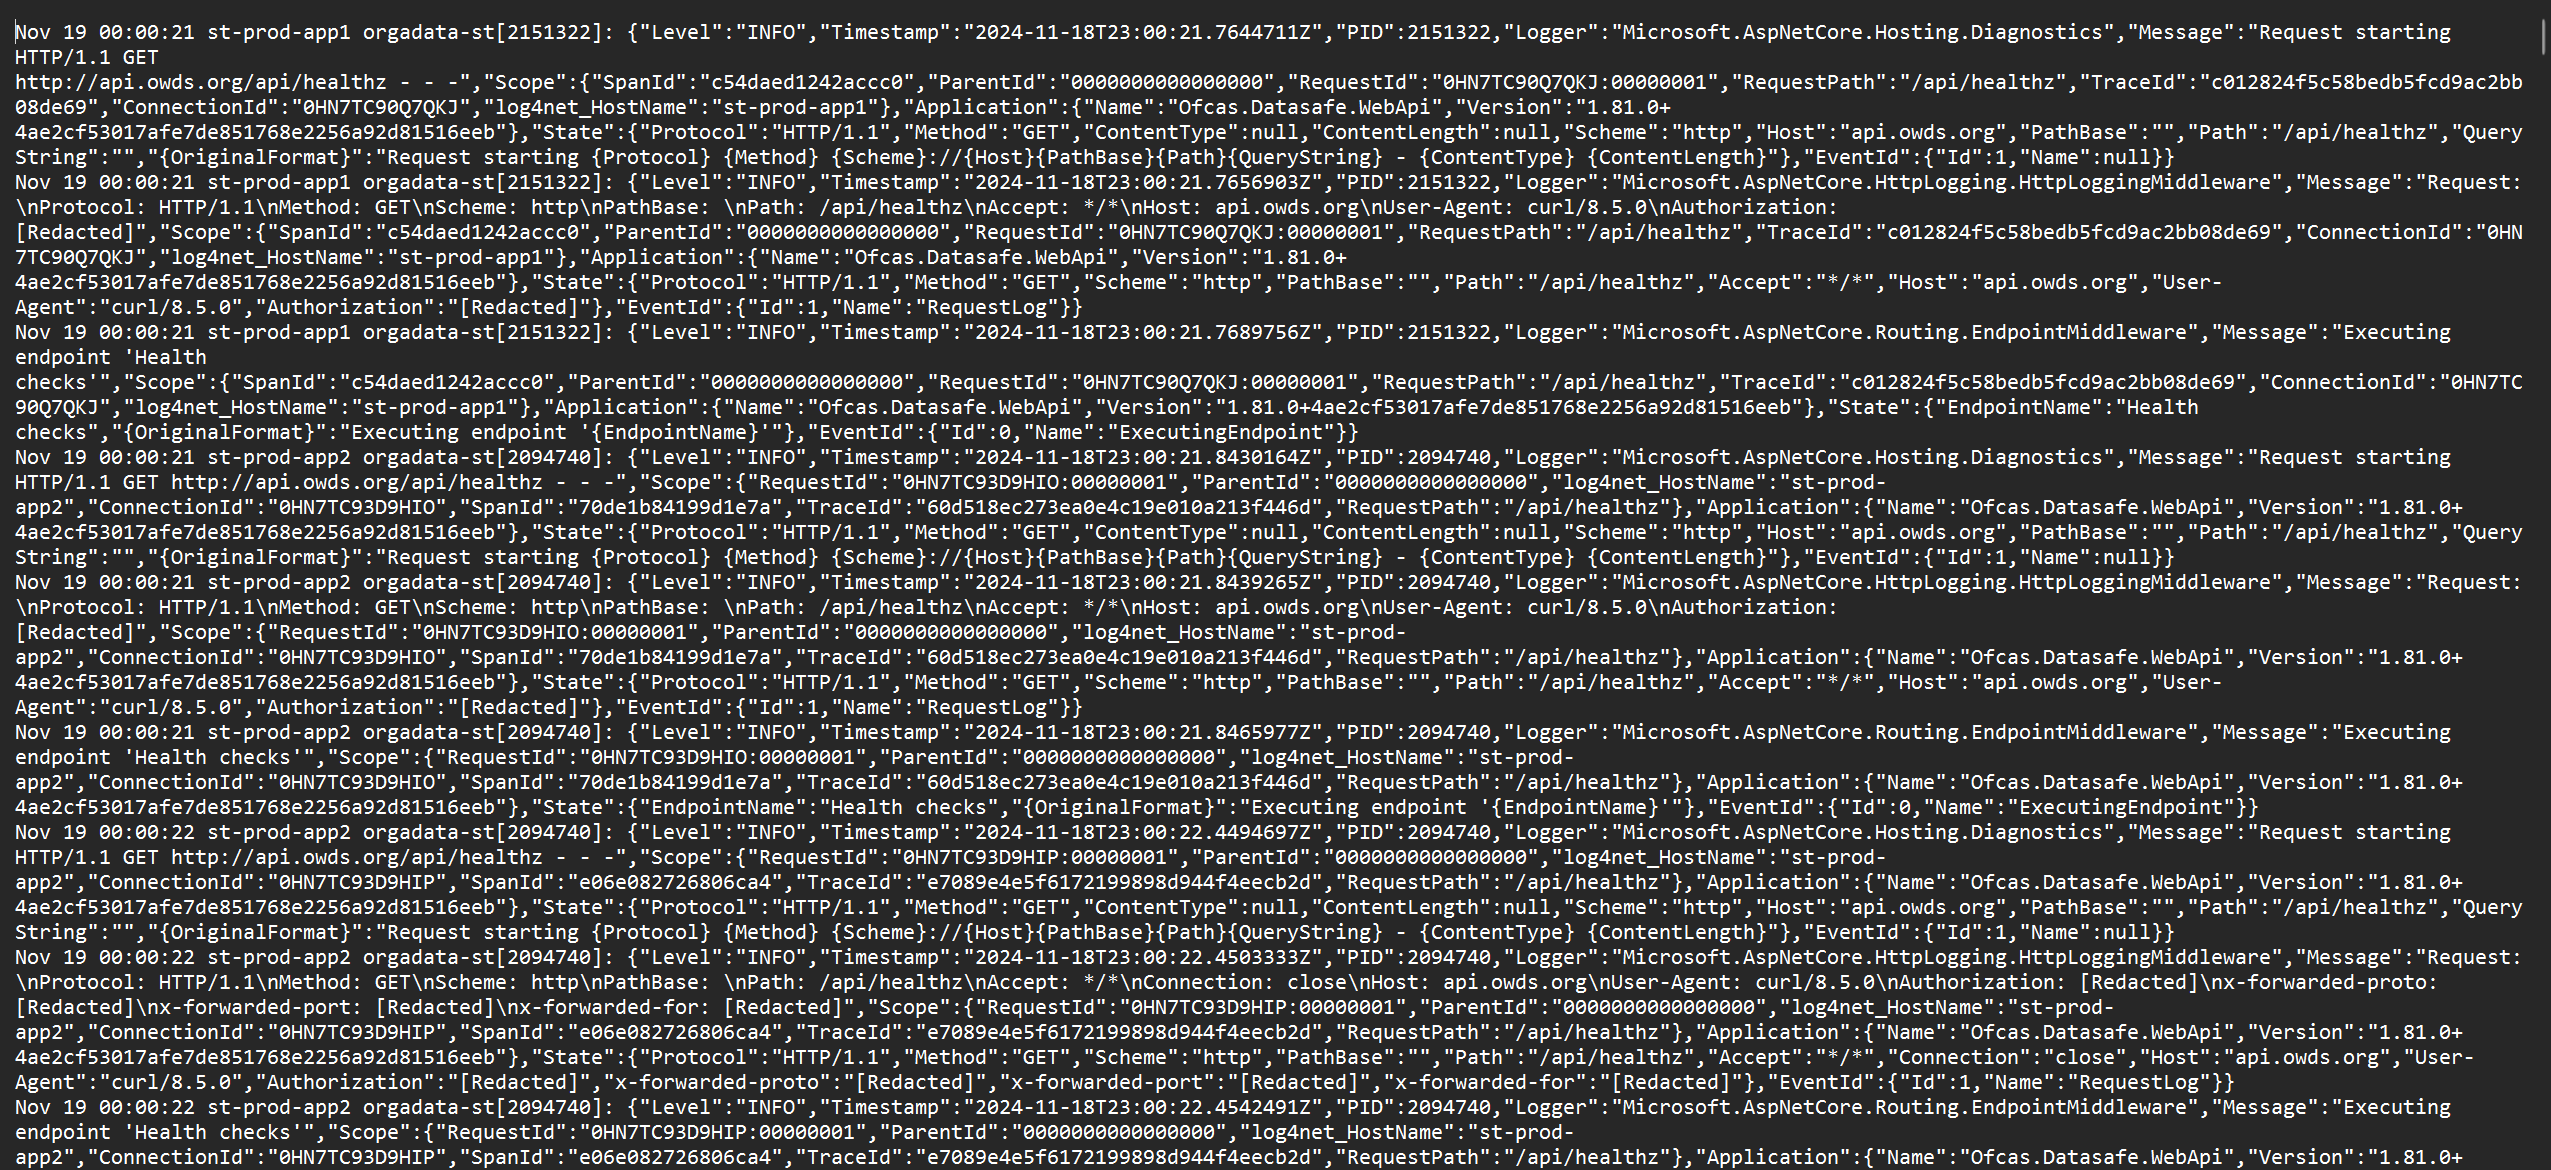
\includegraphics[width=0.7\linewidth]{Images/Data_Img.png}
		\caption{Original Data format}
		\label{Data_Img} 
	\end{center}
\end{figure}

\textbf{Challenges:}
\begin{itemize}
	\item Handling large-scale logs to pinpoint anomalies as shown in the figure ~\ref{Data_Img}.
	\item Differentiating legitimate user activity from malicious attempts.
	\item Establishing efficient protocols to respond to detected threats.
\end{itemize}

\textbf{Results Achieved:}
\begin{itemize}
	\item Implementation of enhanced monitoring protocols using trace IDs and HTTP status codes.
	\item Reduced data breaches by identifying and blocking unauthorized requests.
\end{itemize}

\chapter{Positioning our Analytics}

%\section{Existing Solutions}

%The analytics developed for Orgadata’s SimplyTag system are positioned uniquely when compared to conventional tools. Traditional solutions like Intrusion Detection Systems (IDS) \cite{IEEE:2020} and log monitoring platforms (e.g., Splunk, ELK Stack) \cite{IEEE:2022} offer general frameworks for detecting anomalies and breaches. However, they often lack customization tailored to specific applications. Orgadata’s approach is distinguished by its precise utilization of trace IDs, HTTP status codes, user agent patterns, and paths to monitor requests in real-time.

\section{State-of-the-Art}

\subsection{Overview of Current Solutions}
\begin{itemize}
	\item Existing tools such as Splunk, ELK Stack \cite{IEEE:2022} and Intrusion Detection Systems (IDS) \cite{IEEE:2020} provide robust frameworks for monitoring and analyzing security events. These solutions excel at processing vast amounts of log data and identifying potential threats in general scenarios.
	\item Security platforms often use rule-based or heuristic approaches for anomaly detection but may struggle with domain-specific customizations.
\end{itemize}

\subsection{Capabilities and Limitations}
\begin{itemize}
	\item \textbf{Capabilities:} Tools like Splunk and ELK Stack provide scalability, integration options, and comprehensive dashboards for security analytics. IDS focuses on real-time threat detection.
	\item \textbf{Limitations:}  Lack of precise tailoring for SimplyTag’s requirements, such as analyzing specific HTTP status codes and user agent patterns. High false-positive rates and inability to integrate seamlessly with Orgadata’s infrastructure are additional challenges.
\end{itemize}

\subsection{Relevance to Analytics}

The SimplyTag analytics focus on filling these gaps by leveraging domain-specific insights, such as monitoring trace IDs and HTTP response patterns to identify anomalies and unauthorized activity.

\begin{enumerate}
	\item The use of trace IDs enables seamless tracking of individual requests across logs, allowing for detailed insights into potential vulnerabilities.
	\item By monitoring HTTP status codes, the system identifies and flags suspicious patterns, such as unexpected 200 codes for unauthorized paths.
	\item Integration of user agent analysis ensures that illegitimate devices or configurations can be quickly identified and addressed.
\end{enumerate}

% Suppress page break for the next chapter
\begingroup
\let\cleardoublepage\relax
\let\clearpage\relax
\chapter{Knowledge Domain / Application Sector}
\endgroup

\section{Knowledge domain}

The domain of our analytics is centered around the construction software industry for digital tools and software solutions. By processing system log data from Orgadata's SimplyTag platform, our analytics provide critical insights into system vulnerabilities and anomalies. These insights are invaluable to various functional units, such as IT security teams and system administrators, within the construction software sector, with a focus on:

\begin{itemize}
	\item \textbf{Threat Detection:} Monitoring system logs to identify malicious activity and unauthorized data access.
	\item \textbf{Data Integrity Assurance:} Safeguarding construction-related data from breaches to ensure accurate and reliable information.
	\item \textbf{Operational Security Optimization:} Enabling proactive measures to address potential weaknesses and improve system resilience.
\end{itemize}

By contributing to the broader domain of secure digital tools and software solutions, the project aligns with emerging trends like data-driven operational efficiency and advanced cybersecurity measures tailored for industry-specific applications.

\chapter{Purpose of our Analytics}

\section{What It Does}

This project belongs to the Industry domain, specifically the Construction Software sector, with a focus on:

\begin{itemize}
	\item \textbf{Condition Monitoring:} Tracks HTTP requests in real-time to identify anomalies. This includes analyzing user agents and status codes to pinpoint irregularities that could indicate potential breaches or vulnerabilities.
	\item \textbf{Prevention:} Identifies and blocks malicious requests before they lead to breaches. Proactive security measures ensure that sensitive data and system integrity remain uncompromised.
	\item \textbf{Diagnosis:} Conducts post-incident analysis to refine future detection capabilities. By learning from past incidents, the analytics evolve to handle emerging threats more effectively.
	\item \textbf{Optimization:} Enhances system performance by ensuring secure operations without disrupting user experience. This involves balancing security measures with system usability, especially in high-demand environments like construction software solutions.
\end{itemize}

\begin{figure}
	\begin{center}
		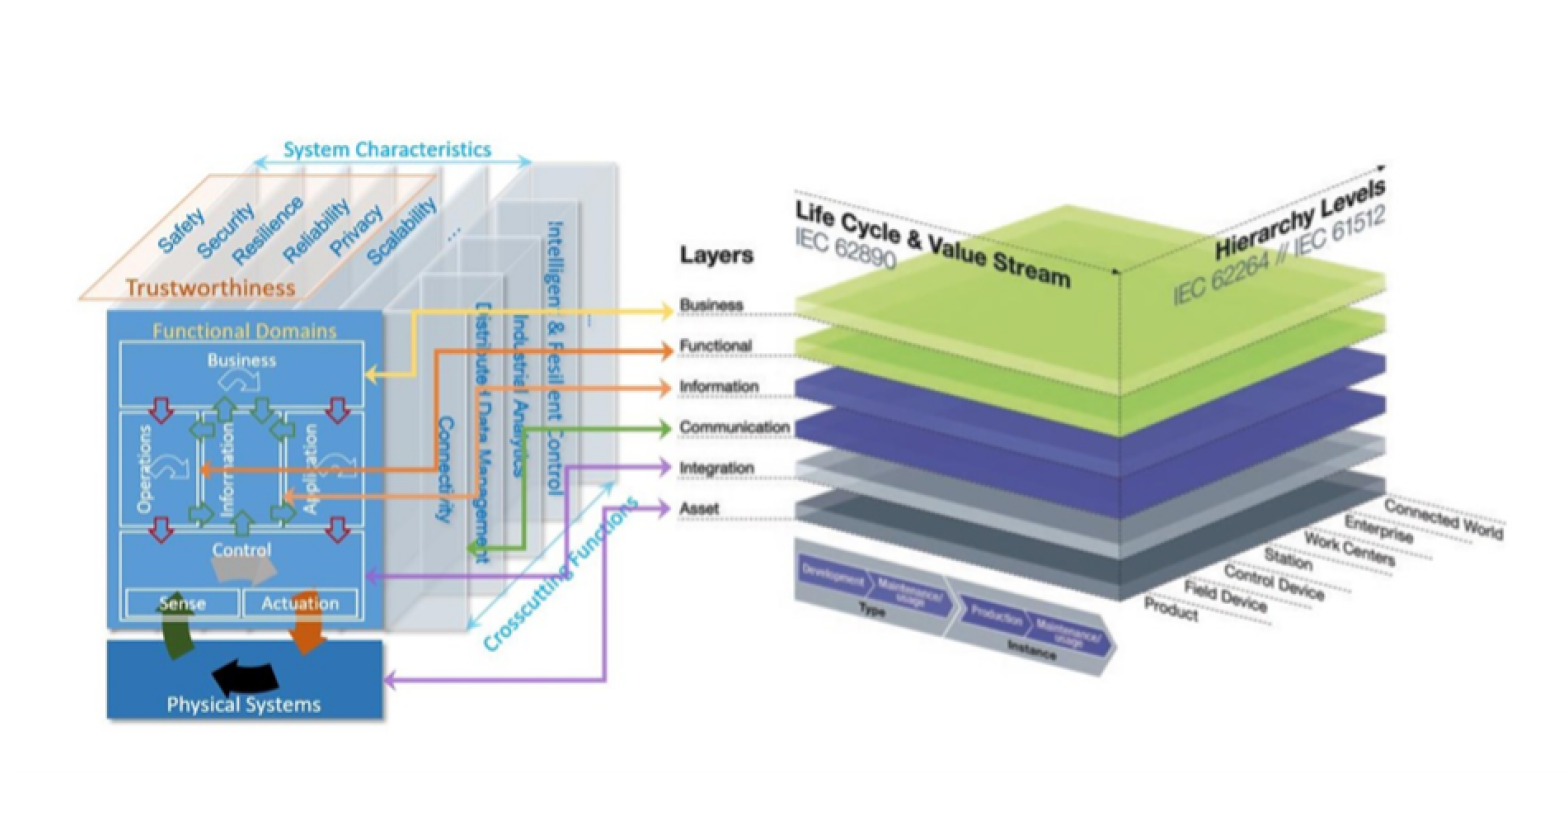
\includegraphics[width=0.7\linewidth]{Images/RAMI_IIRA.png}
		\caption{Mapping Functionalities in RAMI 4.0 and IIRA}
		\label{RAMI_IIRA}
	\end{center}
\end{figure}

\chapter{Positioning Within Standard Reference Architectures}

This solution aligns with several modern frameworks and architectures:

\begin{itemize}
	\item \textbf{Smart-City:} The analytics align with secure data handling standards in urban development contexts, ensuring efficient and secure information exchange in large-scale urban projects..
	\item \textbf{IIoT/IIRA:} The approach supports reliability and security within industrial systems, adhering to frameworks like the Industrial Internet Reference Architecture (IIRA) for seamless integration and operational consistency, refer figure ~\ref{RAMI_IIRA}.
	\item \textbf{RAMI 4.0:} Within the Reference Architecture Model for Industry 4.0 (RAMI 4.0), the analytics are positioned in the \SHELL{"Information Layer"}, where data processing, analysis, and anomaly detection occur. It also contributes to the "Functional Layer" by enabling actionable insights and decision-making based on real-time monitoring, refer figure ~\ref{RAMI_IIRA}.
	\item \textbf{ISO Standards Compliance:} The analytics are developed in alignment with international standards such as ISO 27001, ensuring robust security practices and data protection.
	\item \textbf{Cybersecurity Frameworks:} Incorporating principles from the NIST Cybersecurity Framework, the analytics bolster detection, prevention, and response mechanisms for threats.
\end{itemize}

These alignments ensure that SimplyTag analytics not only address Orgadata’s specific needs but also conform to global benchmarks, making them scalable and applicable across various industrial and urban contexts.

\chapter{Connected Infrastructure Components}

\section{Infrastructure Integration}

\begin{itemize}
	\item \textbf{SimplyTag API Backend:} Serves as the primary source for log data. It collects and provides detailed information about HTTP requests, including trace IDs and status codes, for analysis.
	\item \textbf{Orgadata’s Logikal System:}Acts as the operational backbone for data-driven decision-making. This system contextualizes log data by linking it with construction-related project details, enabling precise threat detection.
	\item \textbf{External Threat Detection Tools:} To enhance the analytics, integration with external tools such as SIEM platforms or advanced machine learning models for threat prediction can be implemented. These tools offer additional layers of analysis and improve overall system resilience.
	\item \textbf{Cloud Infrastructure:} SimplyTag leverages cloud infrastructure to ensure scalability and reliability. The cloud platform supports large-scale log storage and computational power required for real-time analytics.
	\item \textbf{Mobile and Web Interfaces:} The analytics extend to user-facing interfaces like the SimplyTag mobile and web apps, ensuring seamless user interaction while maintaining robust security measures.
\end{itemize}

By connecting these components, the analytics create a comprehensive security ecosystem that is robust, scalable, and aligned with Orgadata’s operational goals.

\chapter{Major Requirements}
\section{Requirements}

\begin{itemize}
	\item \textbf{Structural:} The analytics must seamlessly integrate with existing SimplyTag and Orgadata infrastructure.
	\item \textbf{Behavioral:} Real-time anomaly detection with high accuracy and minimal false positives.
	\item \textbf{Functional:} Efficient parsing of HTTP status codes and trace IDs to identify suspicious activity.
	\item \textbf{Technological:} Implementation of advanced algorithms for log analysis and anomaly detection.
\end{itemize}

This structured approach ensures that the Threat and Weakness Analysis for Orgadata’s SimplyTag system is robust, effective, and well-positioned within industry standards.

